\chapter{Lecture 13 Least Squares Curve Fitting}
\label{ch:lec13n}
\section{Objectives}
The objectives of this lecture are to:
\begin{itemize}
\item Derive the basic formulas for least squares curve fitting.
\item Do an example using MATLAB.
\end{itemize}
\setcounter{lstannotation}{0}

\section{Introduction}
As an engineer, it is very likely that at some point in time during your career,
you will be called upon to examine and interpret experimental data.  Two
common needs in such analysis are to take a set of experimental data and either:
\begin{enumerate}%[label=\alph*.)]
\item develop a model to represent the data. i.e. find a best fit line (or
  other function) through
  the data; or
\item evaluate the data to determine how well it agrees with some previously
  defined model.  i.e. fit model parameters to the data and assess how well
  the experimentally determined values conform to model expectations.

\end{enumerate}

As an example, we will perform a data-fitting analysis of some wind-tunnel
results as presented in a popular numerical methods textbook.\cite[-1.5cm]{gilat} The behavior that we will explore is the dissipation of vortices shed from the tips and trailing
edges of an airfoil in the wind tunnel.  For this example, the tangential
velocity $\left(V_{\theta}\right)$ of a vortex is measured as it travels down the axis of a
wind-tunnel.  The data is non-dimensionalized by dividing the tangential
velocity of the vortex by the free-stream velocity $\left(V_{\infty}\right)$ and by dividing the vortex
position $\left(R\right)$ relative to the airfoil by the chord-length $\left(C\right)$ of the airfoil.  This non-dimensionalization process will allow experimenters to correlate the results from one particular experiment to larger scale tests on geometrically similar prototypes.  The raw data is given in Table \ref{tab:lec13n-numData} and is shown graphically in Figure \ref{fig:lec13n-theData}.
\begin{marginfigure}[-2.5cm]
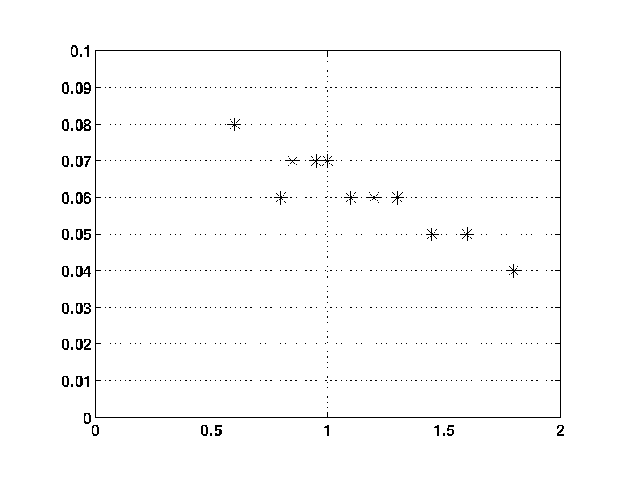
\includegraphics{lec13n_TheData.eps}
\caption{Experimental data from wind tunnel testing.  The $y$-axis is the
  ratio of the tangential velocity of a vortex to the free stream flow
  velocity $\left( y = \sfrac{V_{\theta}}{V_{\infty}}\right)$.  The $x$-axis is
  the ratio of the distance from the vortex core to the chord of an aircraft
  wing. $\left(x = \sfrac{R}{C}\right)$.}
\label{fig:lec13n-theData}
\end{marginfigure}
\begin{table}[h]
\centering
\begin{tabular}{|l|*{11}{c}|}
\hline
$x = \sfrac{V_{\theta}}{V_{\infty}}$ & 0.6 & 0.8 & 0.85 & 0.95 & 1.0 & 1.1 &
  1.2 & 1.3 & 1.45 & 1.6 & 1.8 \\
\hline
$y = \sfrac{R}{C}$ & 0.08 & 0.06 & 0.07 & 0.07 & 0.07 & 0.06 & 0.06 & 0.06 & 0.05 &
  0.05 & 0.04 \\
\hline
\end{tabular}
\caption[][1.5cm]{Numerical data from wind-tunnel experiment.}
\label{tab:lec13n-numData}
\end{table}
In the following sections, we will explore ways in which curves can be fit through this data which, in some sense, are the ``best''-fit curves.

\section{``Guessed''-fit Curves}
It is entirely reasonable, and completely in accord with time honored engineering tradition, to take experimental data as presented in the previous section, use careful judgment and intuition and draw a line that seems to fit the data reasonably well. We will call this the \emph{Guessed}-fit curve and an example of this is shown in Figure \ref{fig:lec13n-guessedfit}.

\begin{marginfigure}
\includegraphics{GuessedFit.eps}
\caption{\emph{Guessed}-fit linear estimation of the experimental data.  $M =
  -0.033$ is the measured slope of the estimated line and $b = 0.1$ is the $y$-intercept.}
\label{fig:lec13n-guessedfit}
\end{marginfigure}  

From this carefully drawn line we may conclude that experimental results show a linear
relationship between tangential velocity and distance downstream from the
airfoil.  Obviously, this model is not perfect; most data-points are off the
line.  Still, we may reasonably decide that overall, this is not a bad
representation of what the data are telling us and leave well enough alone.

\section{Measure of Fitness}

A hand-drawn curve may be well enough for rough analysis, but for the purposes of this lecture, let us assume that we would like to know how good our roughly drawn curve is and wonder if there may be a way to do better.  We have a good fit; but how good is it?  In this section we will answer that question.  We will define a \emph{measure of fitness} so that we may quantitatively determine how ``good'' a candidate curve is in representing the data.

 
For this purpose, we define the \emph{residual}.  In words, the residual $(r_i)$ is the
difference, at each experimental data point $(x_i)$, between the $y$-value given from experimental data $(y_i)$ and the $y$-value computed from our linear ``guessed'' fit curve $\left(y_{\text{guessed}}\right)$.  The mathematical expression for this is given in Equation \ref{resid}.

\begin{equation}
r_{i} = y_{i} - \underbrace{\left(b + Mx_{i}\right)}_{y_{\text{guessed}}} \ \ i = 1,2,\dots,n
\label{resid}
\end{equation}
where $b$ is the $y$-intercept of this linear fit and $M$ is the slope of
the linear fit through the data
and $n$ is the number of data points.

With an eye towards a more general approach, we will re-state Equation \ref{resid} using matrix-vector notation in Equation \ref{residV2}.

\begin{equation}
\begin{split}
\mathbf{r} &= \mathbf{y} - \underbrace{\left( b \cdot \mathbf{x}^0 + M \cdot
\mathbf{x}^{1}\right)}_{\mathbf{y}_{\text{guessed}}} \\
 &= \mathbf{y} - 
\left[
\begin{matrix}
\mathbf{x}^{0} & \mathbf{x}^{1}
\end{matrix}
\right]
\left[
\begin{matrix}
b \\
M
\end{matrix}
\right] \\
&= \mathbf{y} - \mathbf{X}\mathbf{c}
\end{split}
\label{residV2}
\end{equation}

To be clear, please note that $x^{k}$ refers to element-wise exponentiation and in particular, $\mathbf{x}^{0}$ means: ``each element of $\mathbf{x}$ raised to the power of zero,'' and $\mathbf{x}^{1}$ means: ``each element of $\mathbf{x}$ raised to the first power.''  

In order to determine how well a given curve fits the data, the residual given in Equation \ref{residV2} is not quite satisfactory; it is a vector, not a number.  The usual solution to this problem is to use the Euclidean length of the residual as shown in Equation \ref{norm2Resid}:

\begin{equation}
\begin{split}
||r|| &= \sqrt{\mathbf{r}^{T} \mathbf{r}} \\
 &= \sqrt{\sum_{i=1}^{n} r_{i} \cdot r_{i}} 
\end{split} 
\label{norm2Resid}
\end{equation}

For historical reasons, we will depart from this convention and use the ``Euclidean length squared,'' or simply the square of the residual.  We show this in Equation \ref{residSquared} where we also explicitly expand $\mathbf{r}$ as defined in Equation \ref{residV2} to show the residual in terms of the given data $\mathbf{y}$, the matrix $\mathbf{X}$ of our fitting curve and parameter vector $\mathbf{c}$.

\begin{equation}
\begin{split}
\mathbf{r}^{2} &= \mathbf{r}^{T} \mathbf{r} \\
 &= \left(\mathbf{y} - \mathbf{X}\mathbf{c}\right)^{T}\left(\mathbf{y} -
\mathbf{X}\mathbf{c}\right) \\
&= \mathbf{y}^{T}\mathbf{y} - 2 \mathbf{c}^{T}\mathbf{X}^{T}\mathbf{y} +
\mathbf{c}^{T}\mathbf{X}^{T}\mathbf{X}\mathbf{c} 
\end{split}
\label{residSquared}
\end{equation}

The error measure given in Equation \ref{residSquared} now is a single
non-negative number that will in general be zero only if the fitted line passes exactly through all data points.  This is the measure of fitness that we will use.
Using the given values of $\mathbf{y}$, $\mathbf{X}$ and $\mathbf{c}$ for the
``guessed''-fit curve, we find that $\left(\mathbf{r_{\text{guessed}}}\right)^{2} = 0.0152.$ 

\section{Method of Least Squares}

So far we have naively attempted to fit the data as best as we can by guessing
a linear function that might in some way represent the data.  We have defined
an error measure that confirms our suspicion that our linear curve fit is not
perfect.  It is natural to wonder: is there a line that \emph{best} fits the
data\sidenote{At least ``best'' by some error measure.  Different error measures sometimes yield different answers as to what constitutes ``the best.''} and if so, how do we find it? The answer is \emph{``yes, there is a way to find the best fit line''} and the method to find it is called the method of least squares. 

\subsection{Algebraic Derivation}

The standard algebraic derivation of the method of least squares starts with the squared residual given in Equation \ref{residSquared}.  As you should take a moment to confirm, once we have selected a linear estimator\sidenote{
i.e. we have chosen what functions will be used to make up the columns of
$\mathbf{X}$---for the time being we decided it would be composed of the 0\textsuperscript{th}
and 1\textsuperscript{st} powers of $\mathbf{x}$} $\mathbf{X}$, the only free parameter in Equation
\ref{residSquared} are the coefficients that make up $\mathbf{c}$.  The goal
is to figure out how to choose $\mathbf{c}$ such that the error given in
Equation \ref{residSquared} is as small as possible.

Recall from your introductory calculus courses that the way to minimize a
function is to take the first and second derivative of the function; solve for
the values of the free parameter $(\mathbf{c})$ so that the first derivative
is equal to zero; and verify that the second derivative is positive.  When the
first derivative is zero, the function is at an extremum; when the second
derivative is positive, that extremum is a minimum.

Carrying out this idea, we will take the derivative of Equation
\ref{residSquared} and set the first derivative equal to zero:

\begin{equation}
\begin{split}
\frac{d}{d\mathbf{c}}\mathbf{r}^{2} = 0  - 2\mathbf{X}^{T}\mathbf{y} + \underbrace{\mathbf{X}^{T}\mathbf{X}\mathbf{c} + \mathbf{c}^{T}\mathbf{X}^{T}\mathbf{X}}_{\mathbf{X}^{T}\mathbf{X}\mathbf{c} = \mathbf{c}^{T}\mathbf{X}^{T}\mathbf{X}} &= 2\left(-\mathbf{X}^{T}\mathbf{y}+
\mathbf{X}^{T}\mathbf{X} \mathbf{c}\right) = 0 \\
&\Rightarrow -\mathbf{X}^{T}\mathbf{y} + \mathbf{X}^{T}\mathbf{X}\mathbf{c} =
0 \\
&\Rightarrow \mathbf{X}^{T}\mathbf{X} \mathbf{c} = \mathbf{X}^{T}\mathbf{y}
\end{split}
\label{normalEq}
\end{equation}

We now have to ask: can we find a unique vector $\mathbf{c}$ such that the
last line in Equation \ref{normalEq} is satisfied?  The answer is:
yes---provided only that the columns of $\mathbf{X}$ are linearly
independent,\sidenote{If the columns of $\mathbf{X}$ are linearly independent, this means---by definition---that $\mathbf{Xy} = 0$ if and only if $\mathbf{y}=0$.} $\mathbf{X}^{T}\mathbf{X}$ will be positive-definite and thus non-singular.\sidenote{When a matrix---$\mathbf{A} =
  \mathbf{X}^{T}\mathbf{X}$--- is positive definite, that means that
  $\mathbf{y}^{T}\mathbf{Ay}=0$ if and only if $\mathbf{y}=0$.  So $\mathbf{y}
  \ne 0$ and if the columns of $\mathbf{X}$ are linearly independent ($\mathbf{Xy} \ne 0$),
  then $\mathbf{y}^{T}\mathbf{X}^{T}\mathbf{X}^{T}\mathbf{y} \ge 0$ and can
  \emph{only} be equal to zero if $\mathbf{y}=0$.  As is discussed in
  in previous lectures, positive-definiteness is a sufficient condition for a solution to Equation
  \ref{normalEq} to exist.}  This means that a unique value of $\mathbf{c}$
will exist and that it will be non-zero:

\begin{equation}
\mathbf{c} = \left(\mathbf{X}^{T}\mathbf{X}\right)^{-1}
\left(\mathbf{X}^{T}\mathbf{y}\right)
\label{lstSqSol}
\end{equation} 


MATLAB code to carry out this process is given below:

\begin{lstlisting}[style=myMatlab]
x = [0.6 0.8 0.85 0.95 1.0 1.1 1.2 1.3 1.45 1.6 1.8]; 
y = [0.08 0.06 0.07 0.07 0.07 0.06 0.06 0.06 0.05 0.05 0.04]; 

X = nan(length(x),2);
X(:,1) = (x').^0;
X(:,2) = (x').^1;

c = (X'*X) \ (X'*y');
\end{lstlisting}

Executing this code with our given data we solve for $\mathbf{c}$ which gives
us the $y$-intercept and slope of a different linear curve for the data which we will tentatively call the ``best'' linear fit. The resulting line is presented along with the previous ``guessed''-fit curve
for comparison in Figure \ref{fig:lec13n-bestFitPlot}.  Using Equation \ref{residSquared}, we find that the squared residual of this solution is: 0.0140 which is slightly better than our previous ``guessed''
estimate of 0.0152.

\begin{marginfigure}
\includegraphics{BestFit.eps}
\caption{Best fit linear estimation of the experimental data.  $M =
  -0.0288$ is the measured slope of the estimated line and $b = 0.0940$ is the $y$-intercept.}
\label{fig:lec13n-bestFitPlot}
\end{marginfigure}  



The second step is to prove that the coefficient array $\mathbf{c}$ really is a minimum and not a maximum or saddle-point.    One answer is to say that if we, once again, take the derivative of Equation \ref{normalEq}, we get:

\begin{equation}
\begin{split}
\frac{d^{2}}{d \mathbf{c}^{2}}\mathbf{r}^{2} &= \frac{d}{d \mathbf{c}} \left(-\mathbf{X}^{T}\mathbf{y} + \mathbf{X}^{T}\mathbf{X}\mathbf{c}\right) \\
&= \mathbf{X}^{T}\mathbf{X}
\end{split}
\label{secondDeriv}
\end{equation}

The problem with this, is that the last line of Equation \ref{secondDeriv} is not simply a number; it is a matrix. It turns out that if the columns of $\mathbf{X}$ are linearly independent, then the square matrix $\mathbf{X}^{T}\mathbf{X}$ is symmetric and positive definite.  The property of a matrix: ``symmetric, positive definite'' carries with it some implications:

\begin{enumerate}
\item all of the eigenvalues of the matrix are real and positive; and
\item the matrix is invertible
\end{enumerate}

Though it may smack of hand-waving, the author requests your indulgence and accept that these properties carry the same implications as a positive second derivative for the residual function.  The curve found via the method of least squares is, in fact, the curve with the minimum residual; not an inflection point and definitely not the maximum.\sidenote{The existence of the ``guessed''-fit curve with a higher residual than the curve found using the method of least squares should be convincing proof that the method of least squares, at least, does not find the curve with the maximum residual.}


Based on the mathematical results of this section we can
assert that no \emph{linear} estimator of this data set can
achieve a squared residual error of less than 0.0140.

\section{Linear Least Squared with Non-Linear Estimator}

So far, we have accomplished much, but what do we do in the case where we do
not expect the $x$ and $y$ data that we collected in our experiment to be
linearly related?  The answer is a straight-forward
extension of the method of least squares presented in the preceding section.  

Suppose we would like to find the best quadratic fit through the data?  That
is, we are seeking some function: $c_{1} + c_{2}\mathbf{x} + c_{3}
\mathbf{x}^{2}$ such that the squared residual is as small as possible.  All
that we need to do is to re-define $\mathbf{c}$ to accommodate the extra
parameter and re-define $\mathbf{X}$ to incorporate the extra functional dependence on $\mathbf{x}$.  Specifically:

\begin{equation}
\begin{split}
\mathbf{c} &= 
\left[
\begin{matrix}
c_{1} & c_{2} & c_{3} 
\end{matrix}
\right]^{T} \\
\mathbf{X} &= 
\left[
\begin{matrix}
\mathbf{x}^{0} & \mathbf{x}^{1} & \mathbf{x}^{2}
\end{matrix}
\right]
\end{split}
\label{bestQuad}
\end{equation}

We use this newly defined $\mathbf{X}$ and solve for the corresponding values
of $\mathbf{c}$ using Equation \ref{lstSqSol} \emph{exactly as before}.(!!) Nothing in the process need change because, just as with the linear estimator, all that is required is that the columns of $\mathbf{X}$ be linearly independent. To highlight how general this concept is, we will again change our notation slightly and write $\mathbf{X}$ as:

\begin{equation}
\mathbf{X} = 
\left[
\begin{matrix}
f_{1}(\mathbf{x}) & f_{2}(\mathbf{x}) & \cdots & f_{k}(\mathbf{x})
\end{matrix}
\right]
\end{equation}  
where here $k$ is the index of the columns of $\mathbf{X}$.  For the linear case, $f_{1}(\mathbf{x}) = 1$, $f_{2}(\mathbf{x}) = \mathbf{x}$.  For the quadratic case, we simply add $f_{3}(\mathbf{x}) = \mathbf{x}^{2}$.  Each of the functions: $f_{1}$, $f_{2}$ and $f_{3}$ are linearly independent.\sidenote{Here again a definition is worthwhile.  For a set of   functions to be linearly independent it implies that for scalar values   $c_{i}$, $c_{1}f_{1}(\mathbf{x}) + \cdots + c_{k}f_{k}(\mathbf{x}) = 0$ if and only if $c_{1} = \cdots = c_{k} = 0$.  All of the monomials: 1, $x$, $x^2$, etc... as easily seen to be linearly independent.} Taking this a step further, we could use \emph{any} set of linearly independent functions and Equation \ref{lstSqSol} would still have a unique solution that would provide the parameter vector $\mathbf{c}$ such that the squared residual will be as small
as possible.

The process of using high order polynomials to fit data is so common, that MATLAB has a built-in function---polyfit---to automate least-squares estimation with polynomial estimators.  The code block below does this for second order, third order and sixth order polynomials.  The resulting estimators are given in Figure \ref{HighOrderFitPlot}.  

\begin{lstlisting}[style=myMatlab]
x = [0.6 0.8 0.85 0.95 1.0 1.1 1.2 1.3 1.45 1.6 1.8]; 
y = [0.08 0.06 0.07 0.07 0.07 0.06 0.06 0.06 0.05 0.05 0.04]; 
cSecond = polyfit(x,y,2); 
ySecond = cSecond(1)*x.^2 + cSecond(2)*x + ...
    cSecond(3);
cThird = polyfit(x,y,3);
yThird = cThird(1)*x.^3 + cThird(2)*x.^2 + ...
    cThird(3)*x + cThird(4);
cSixth = polyfit(x,y,6);
ySixth = cSixth(1)*x.^6 + cSixth(2)*x.^5 + ...
    cSixth(3)*x.^4 + cSixth(4)*x.^3 + cSixth(5)*x.^2 + ...
    cSixth(6)*x + cSixth(7);
\end{lstlisting}


\begin{marginfigure}[-5.5cm]
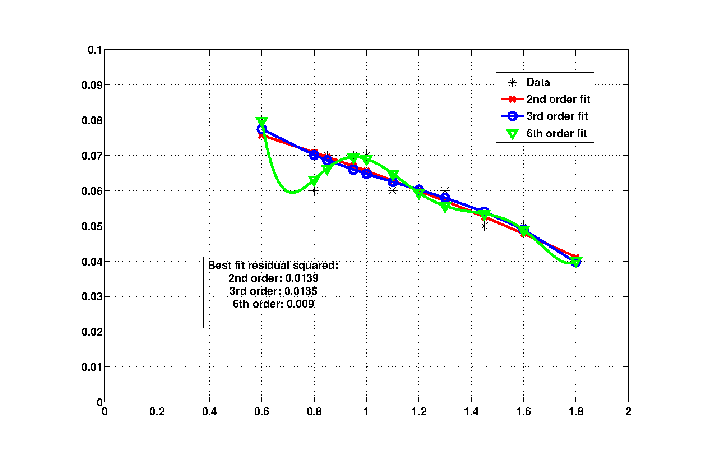
\includegraphics{HigherOrder.eps}
\caption{Best fit linear estimation of the experimental data using 2nd order,
  3rd order and 6th order estimators.}
\label{HighOrderFitPlot}
\end{marginfigure}  

\section{Model Estimators}

As can be seen from Figure \ref{HighOrderFitPlot}, it is possible to find estimators that greatly reduce the squared residual.\sidenote[][-2.5cm]{In general it is possible to find a polynomial that exactly interpolates any number of data points with the resulting residual equal to zero.  It turns out, doing this with polynomial interpolants is usually a very bad idea---at least with ordinary monomials and with equally spaced data points---and when using non-exact floating point arithmetic, and a large number of data points is involved, it is practically impossible.  Better interpolation methods with non-equally-spaced points are almost always used where very accurate interpolation is necessary (for example: when implementing high order finite element methods).}  As higher order estimators are used, the resulting curve through the data becomes problematic.  For example, how would one justify the ``curvy'' nature of the 6th-order approximator?  If we re-performed the experiment with improved instrumentation and made our measurements more carefully, do we \emph{actually} expect the data to follow the 6th order curve?  Probably not.  

It is also worthwhile to consider that the purpose of doing all of this least squares estimation is \emph{not} always to find some curve that comes close to interpolating all of the data.  Rather, the purpose may be to fit the data to a rational scientific model where the experimental data either confirms and strengthens the proposed model for the phenomena under consideration, or serves as the basis for creation of a new model.\cite{trefethen2}

For this example, it turns out that theoretical models do exist regarding the expected vortex velocity as it travels downstream from an airfoil in a wind-tunnel.  This model predicts that the relationship between $y$---the ratio between the vortex tangential velocity and the free-stream velocity---and $x$---the ratio of the distance from the vortex core to the chord of the airfoil section---should have the form of Equation \ref{modelRelation}.

\begin{equation}
y = \frac{A}{x} + \frac{B e^{-2 x^{2}}}{x}
\label{modelRelation}
\end{equation}

As before, we can develop an estimator that conforms with this model in exactly the same way we did for the polynomial estimators.  MATLAB code accomplishing this is provided in the code block below:

\begin{lstlisting}[style=myMatlab]
X = nan(length(x),2);
f1 = @(t) (1./t); % functional form of first term
f2 = @(t) exp(-2*t.^2)./t; % functional form of second term
X(:,1) = f1(x');
X(:,2) = f2(x');
cModel = X\(y');
\end{lstlisting}

Please note a couple of differences between this code and code previously provided:

\begin{enumerate}%[label=\alph*.)]
\item Anonymous functions are used to simplify the construction of
  $\mathbf{X}$.  This is a stylistic choice but could be useful for
  cases where you want automate this process.
\item The usual ``backslash'' left division operator was used instead of the formula specified in Equation \ref{lstSqSol}.  The reason this works is because
  MATLAB automatically checked and noted that $\mathbf{X}$ was not a square
  matrix (normally a requirement for left matrix division); seeing it was
  not square, then it checked to see if each column of $\mathbf{X}$ is
  linearly independent; MATLAB determined that they were and used the equivalent of
  Equation \ref{lstSqSol} to solve for $\mathbf{c}$.\sidenote[][-4.0cm]{The normal
    equations is the easiest method to derive, but actually solving the normal
    equations directly turns out not to be the very best way of finding
    $\mathbf{c}$.}  
\end{enumerate}

The resulting curve, along with the linear estimator is shown in Figure \ref{modelPlot}.


\begin{marginfigure}[-2.0cm]
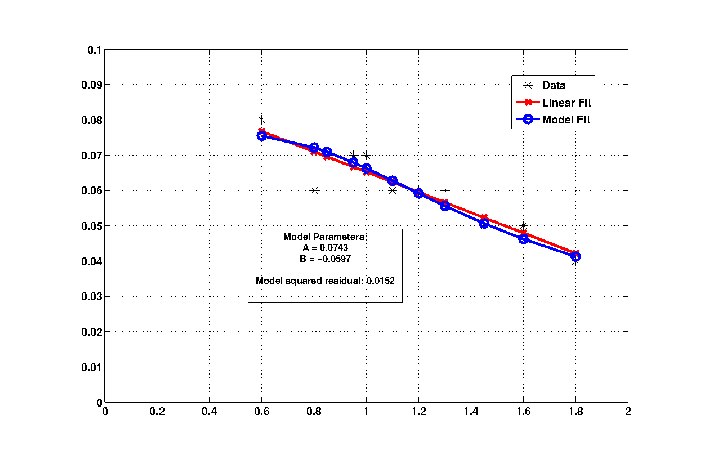
\includegraphics{Model.eps}
\caption{Best fit curve with theoretical model parameters.  The linear Least
  Squares estimator is shown for reference.}
\label{modelPlot}
\end{marginfigure}  


As we can see, the residual squared for the theoretical model estimator is larger than the residual squared for the linear estimator shown previously. Remember, the purpose of fitting a curve through the data points in this context is to gain insight as to how well the recorded experimental data can fit against a known (or proposed) theoretical model.  If we wanted a residual of zero, we could have gotten it through the mechanical process of providing an exact interpolant through the data; but that would hardly yield a reasonable model.  Even though the residual of this new model is higher than for a linear estimator, we gain the benefit of seeing how well the theoretical model stands up in the face of experimental evidence.  

\section{MATLAB Example}

In an electrophoretic fiber-making process, the diameter of the fiber, $d$, is related to the current flow, $I$.  The following measurements are made during production:
\begin{table}[h!]
\begin{tabular}{|l|l|l|l|l|l|l|l|l|l|}
\hline
$I$ (nA) & 300 & 300 & 350 & 400 & 400 & 500 & 500 & 650 & 650 \\ \hline
$d$ ($\mu$m) & 22 & 26 & 27 & 30 & 34 & 33 & 33.5 & 37 & 42 \\ \hline
\end{tabular}
\caption{Process data from electrophoretic fiber-making process.}
\end{table}

\begin{enumerate}
\item Use linear least-squares regression to determine the coefficients $m$ and $b$ in the function $y=mx+b$ that best fits the data.
\item Use least-squares regression to determine the coefficients $a$, $b$, and $c$ in the function $y = a + bx + cx^2$.
\item Use least-squares regression to determine the coefficients $a$ and $b$ in the function $y = a + b\sqrt{I}$.
\end{enumerate}

We start, as always, by clearing out the workspace and command window and closing any open figure windows.  We will also input the given data.
\begin{lstlisting}[style=myMatlab,name=lec13n-ex1]
clear
clc
close 'all'

%% Input Data
I = [300 300 350 400 400 500 500 650 650]';
d = [22 26 27 30 34 33 33.5 37 42]';

\end{lstlisting}

The linear least-squares regression is carried out in the following code; the best fit line is shown in Figure \ref{fig:lec13n-ex1-linear-fit}
\begin{marginfigure}
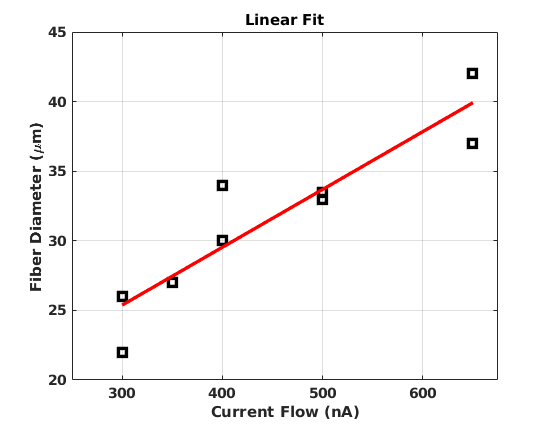
\includegraphics{lec13n-ex1-linear-fit.png}
\caption{Linear fit, $m=0.416$, $b=12.913$.}
\label{fig:lec13n-ex1-linear-fit}
\end{marginfigure}
\begin{lstlisting}[name=lec13n-ex1, style=myMatlab]
X = [ I.^0 I.^1];
b = d;

c = (X'*X)\(X'*b);

linEst = @(x) c(1) + c(2)*x;
\end{lstlisting}
A least-squares regression to fit a second-order polynomial to the data is carried out in the next listing.
\begin{lstlisting}[name=lec13n-ex1,style=myMatlab]
X = [I.^0 I.^1 I.^2];
b = d;

c = (X'*X)\(X'*b);

quadEst = @(x) c(1) + c(2)*x + c(3)*x.^2;
\end{lstlisting}
A plot of the resulting estimator is shown in Figure \ref{fig:lec13n-ex1-second-order-fit}.
\begin{marginfigure}
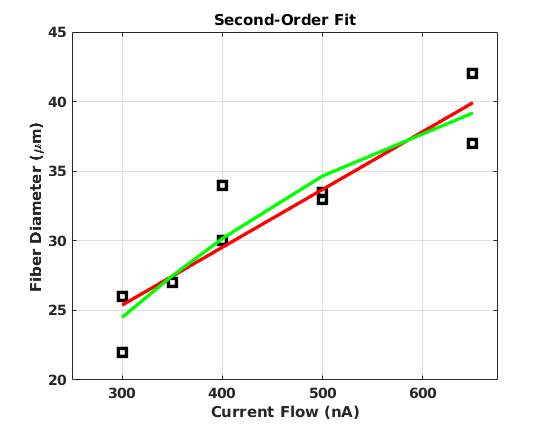
\includegraphics{lec13n-ex1-second-order-fit.png}
\caption{Second-order polynomial fit. $a=0.436$, $b=0.0979$, and $c=-5.89e-5$.}
\label{fig:lec13n-ex1-second-order-fit}  
\end{marginfigure}
Using an estimator like $y = a + b\sqrt{I}$ is accommodated in exactly the same way; there is a constant term---proportional to $I^{0}$---and a term proportional to $I^{\sfrac{1}{2}}$.  The MATLAB code is shown in the listing below and the resulting estimator, along with the previously found estimators, is shown in Figure \ref{fig:lec13n-ex1-model-fit}.

\begin{marginfigure}
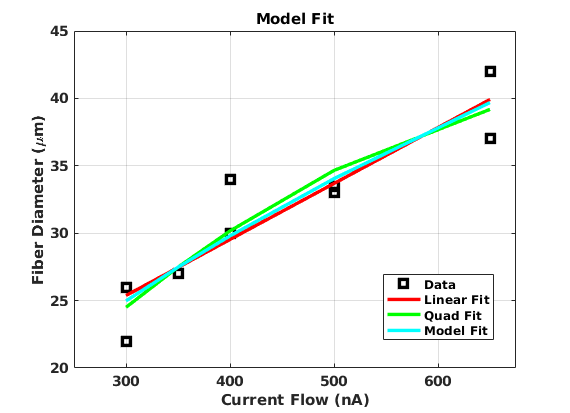
\includegraphics{lec13n-ex1-model-fit.png}
\caption{Model fit of data.  $a = -6.20$, $b=1.80$.} 
\label{fig:lec13n-ex1-model-fit}
\end{marginfigure}

\begin{lstlisting}[style=myMatlab,name=lec13n-ex1]
X = [I.^0 I.^0.5];
b = d;
c = (X'*X)\(X'*b);

est3 = @(x) c(1) + c(2)*x.^0.5;
\end{lstlisting}

